\documentclass[11pt,fleqn]{article}

\setlength {\topmargin} {-.15in}
\setlength {\textheight} {8.6in}

\usepackage{amsmath}
\usepackage{amssymb}
\usepackage{color}
\usepackage{tikz}
\usetikzlibrary{automata,positioning,arrows}
\usepackage{diagbox}



\newcommand{\be}{\begin{enumerate}}
\newcommand{\ee}{\end{enumerate}}

\begin{document}
\begin{center}
	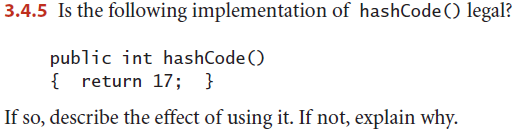
\includegraphics[scale=1]{3.4.5.png}
\end{center}
	
\textbf{Solution:}
Since every item is put in the same position in the hashtable due to same hashcode, it will result in a linkedlist. This is ineffective because everything saved to the same spot so there is no difference between this and a linkedlist. This is basically collision of chaining.

\begin{center}
	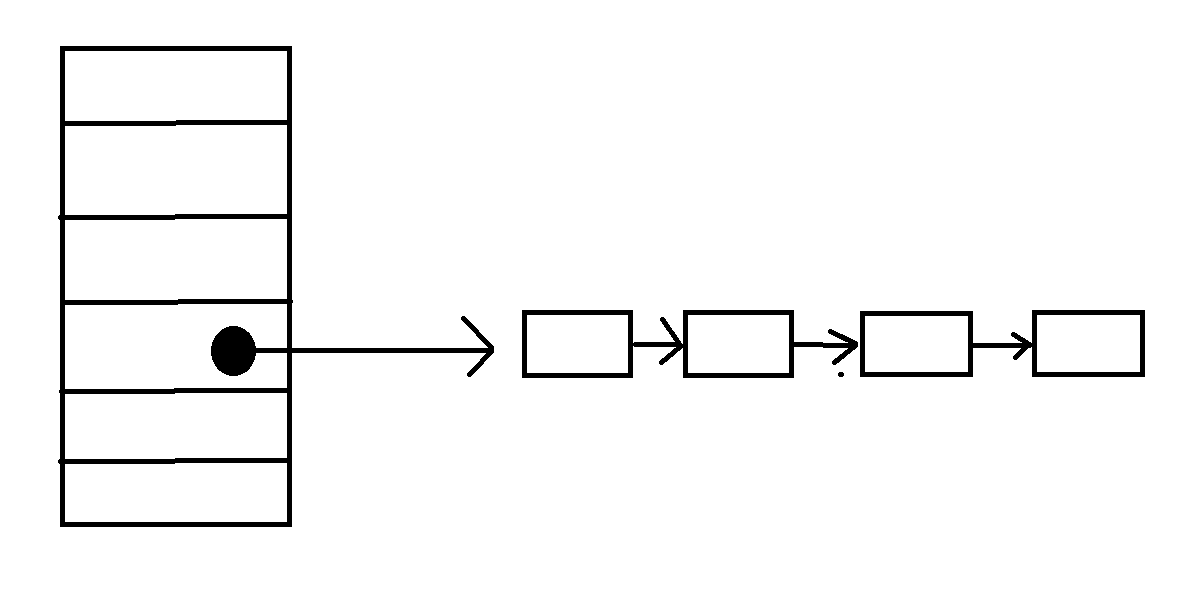
\includegraphics[scale=.44]{3.4.5-soln.png}
\end{center}

\end{document}
